\documentclass[colorlinks=true,pdfstartview=FitV,linkcolor=blue,
            citecolor=red,urlcolor=magenta]{ligodoc}

\usepackage{graphicx}
\usepackage{amssymb}
\usepackage{amsmath}
\usepackage{longtable}
\usepackage{rotating}
\usepackage[usenames,dvipsnames]{color}
\usepackage{fancyhdr}
\usepackage{subfigure}
\usepackage{hyperref}

\title{Optical Contacting - THIS IS NOT THE ENTIRE DOCUMENT}

\author{Jennifer Hritz}

\begin{document}

\section{Appendix \# - Parts List/Experiment Design}

\subsection{Shear strength}

My design was inspired by the apparatus used in a paper which was measuring the shear strength of a glass-glass direct bond \cite{Helie}. The paper had a picture of their apparatus (Figure \ref{fig:apparatus}) but did not explain how their apparatus was constructed---most importantly, they did not explain how they mounted their wafers---so I had to design that myself.

\begin{figure}[htbp]
\begin{center}
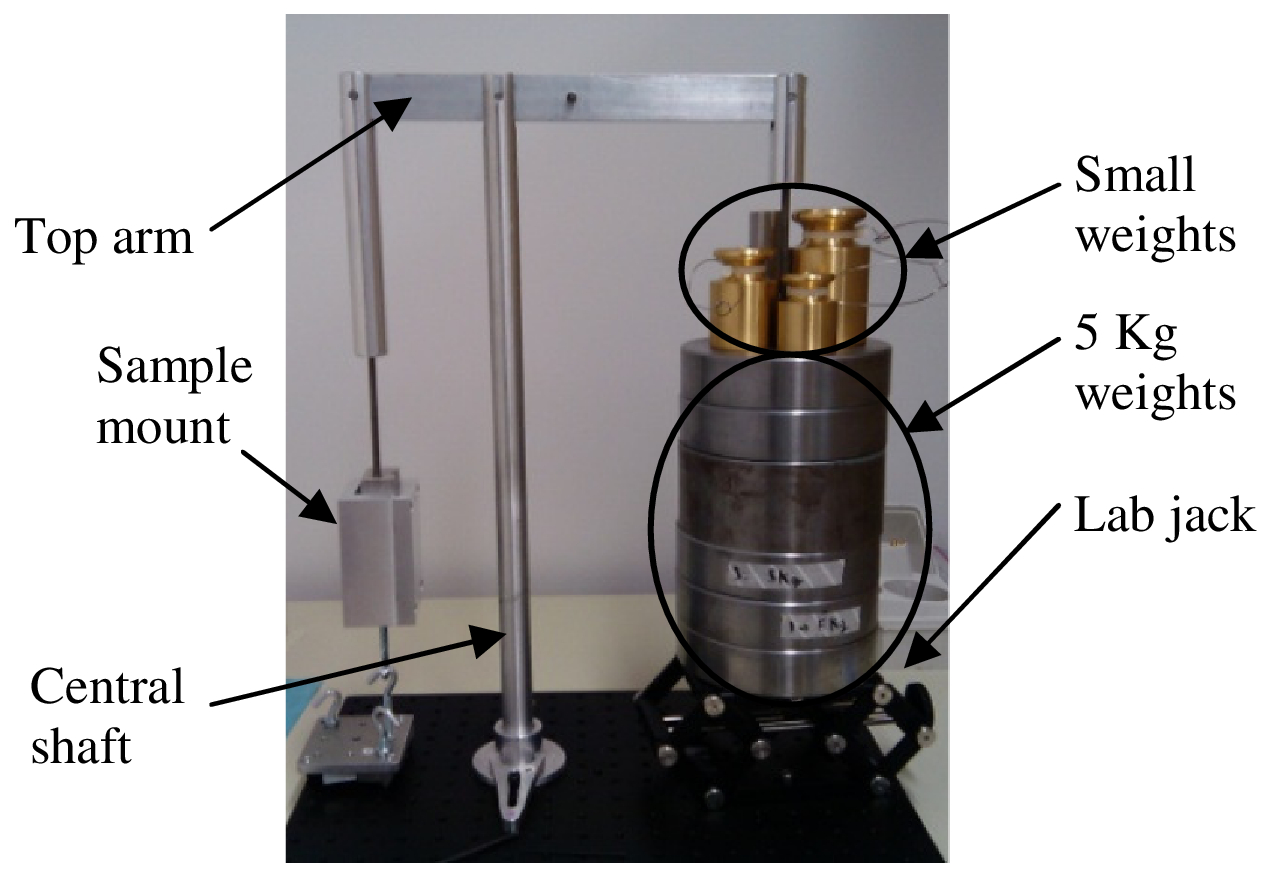
\includegraphics[width=6in]{apparatus.png}
\caption{"Photograph of the setup used for shear strength measurements." \cite{Helie}.}
\label{fig:apparatus}
\end{center}
\end{figure}

The shear strength is measured by mounting the optically bonded wafers on one side of a beam balance then slowly adding weight to the other side until the bond is broken. As shown in Figure \ref{fig:myapparatus}, the bonded wafers are mounted such that weight pulls up one side while the other remains secure. A lab jack is used to assist with adding the weights.

\newpage

\begin{figure}[htbp]
\begin{center}
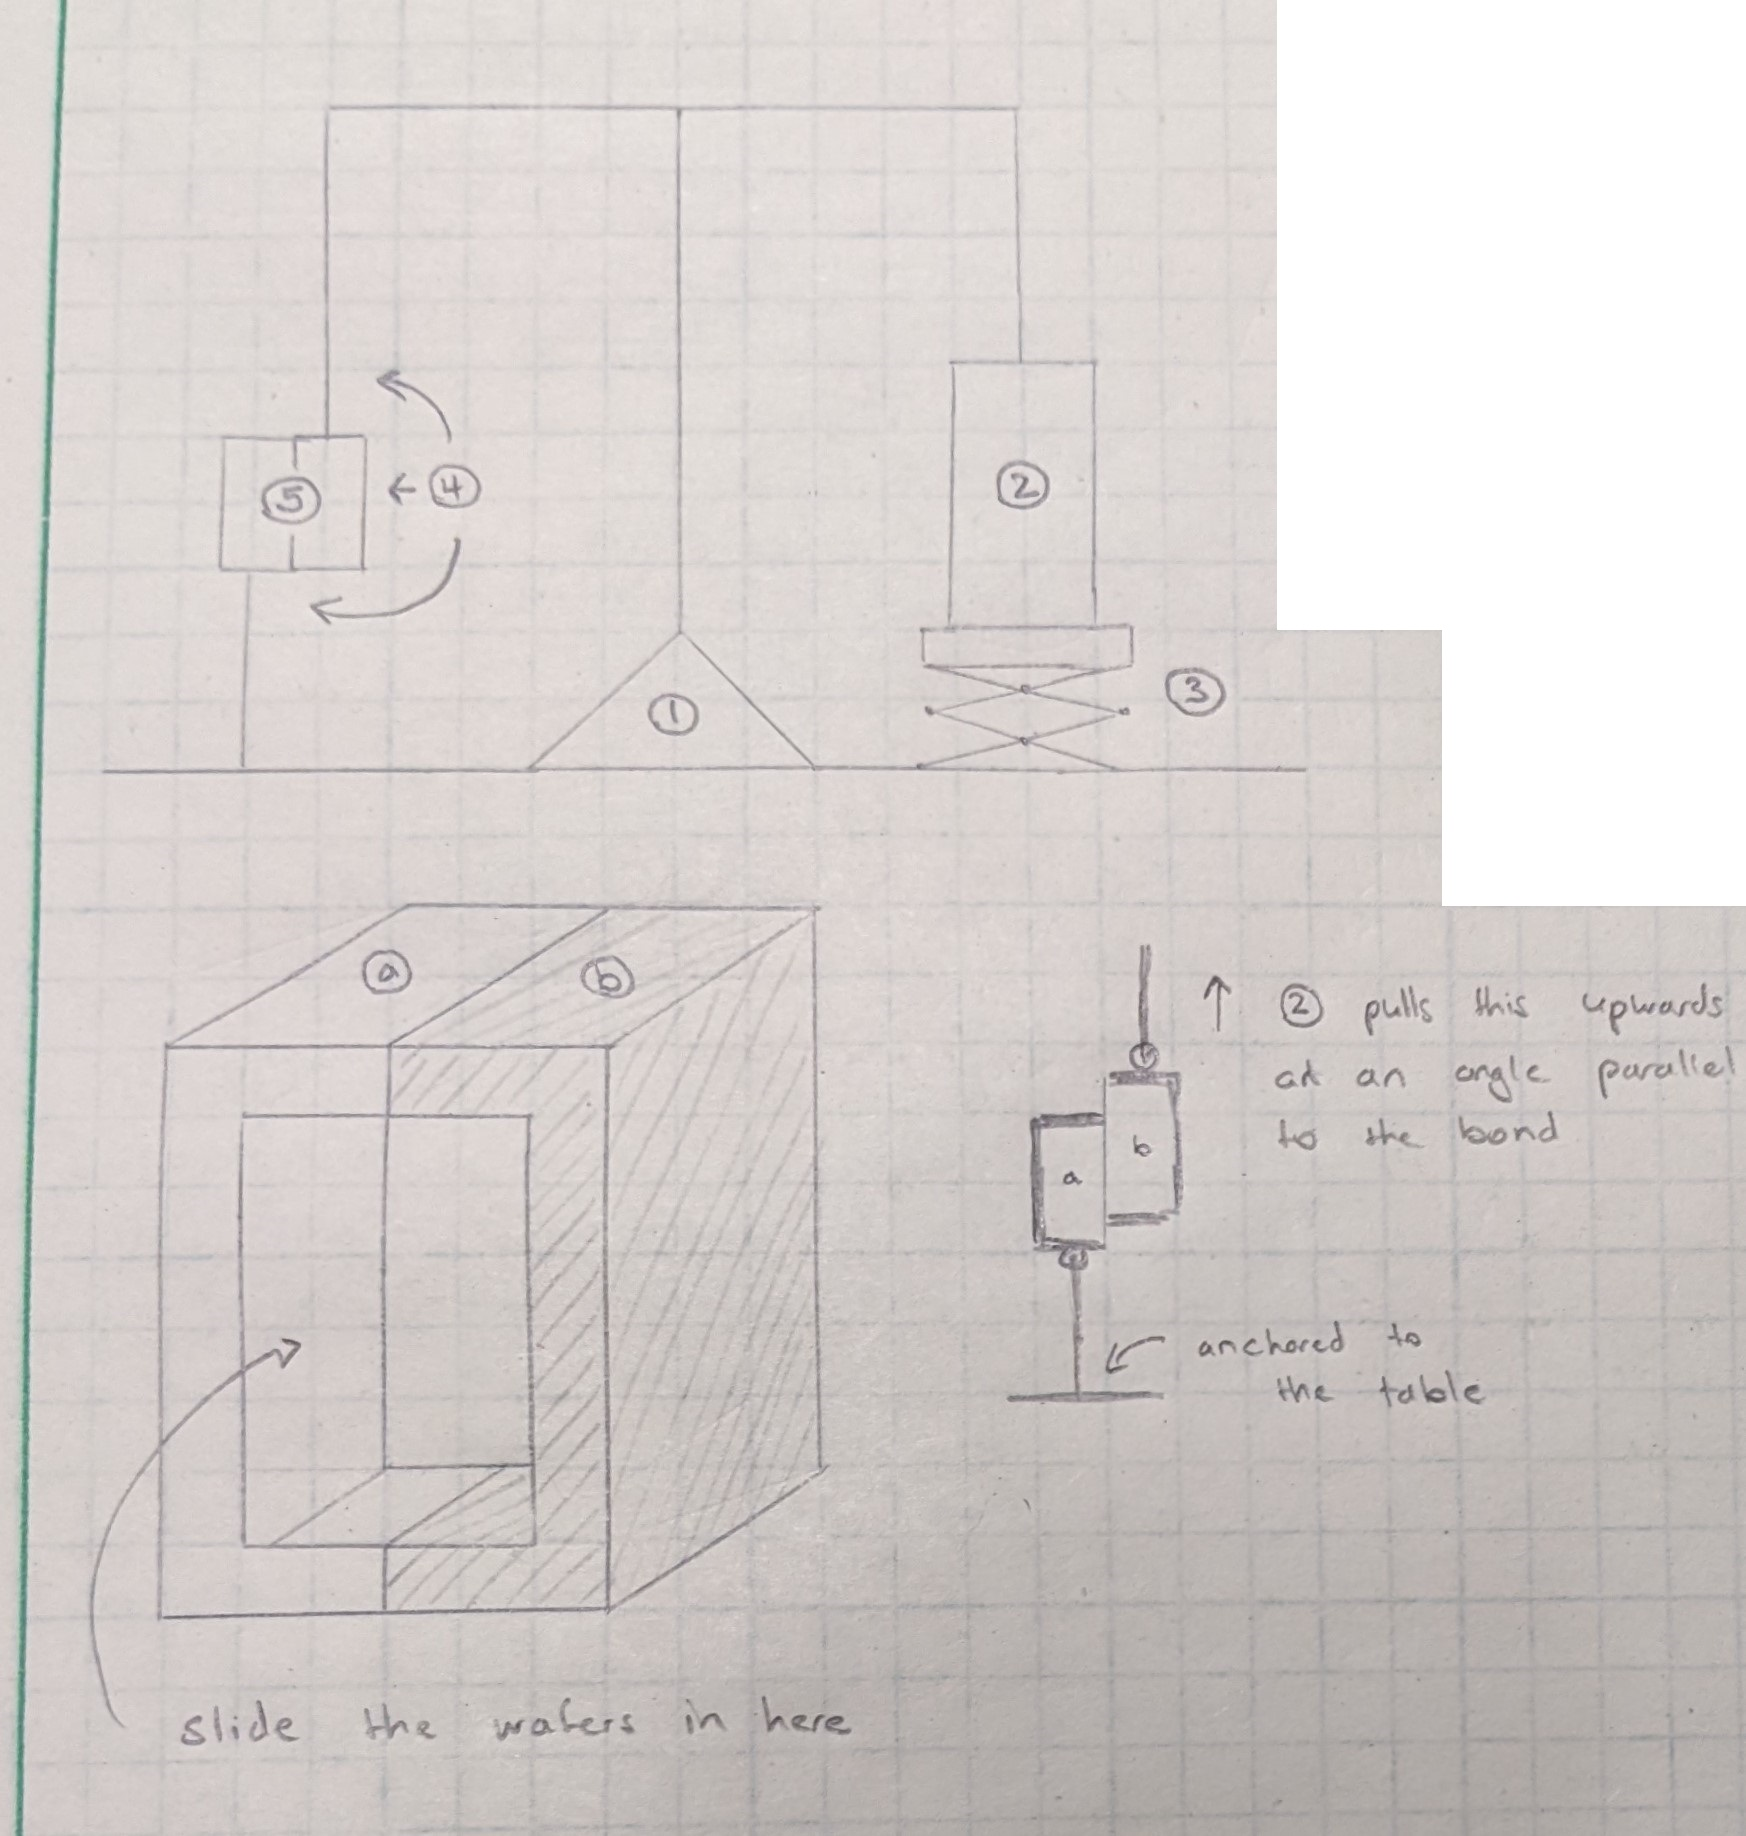
\includegraphics[width=6in]{scratchwork.jpg}
\caption{My design of my apparatus and the mount for the bonded wafers as well as a crude diagram of how the apparatus functions.}
\label{fig:myapparatus}
\end{center}
\end{figure}

\newpage

Parts list:

\begin{enumerate}
  \item Traditional beam balance
    \begin{itemize}
    \item I am not sure if this can be purchased or it will need to be constructed. It seems simple enough to me, but I could be underestimating its complexity.
    \item If it needs to be constructed, I can put together a list of the parts needed.
    \end{itemize}
  \item Various weights (total to roughly 100 kg)
    \begin{itemize}
    \item The idea is to slowly add smaller weights until you reach a certain amount then remove them and add a big single weight equivalent to their weight. Repeat until failure.
    \item I swear I have seen weights like in Figure \ref{fig:apparatus} used in a lab class, so I presume they are not something that needs to be purchased.
    \end{itemize}
  \item Lab jack
    \begin{itemize}
    \item This is for taking the weight off the bonded wafers while replacing the smaller weights with the big single weight.
    \end{itemize}
  \item Mount for bonded wafers
    \begin{itemize}
    \item This was the hardest part to design since it needs to be a snug fit while also being capable of bearing weight. My idea is to 3D print a casing like in Figure \ref{fig:myapparatus}. I am unsure if I can 3D print with a material strong enough to bear the weight, so perhaps metal should be attached around them. The mount is attached to the beam balance with a hook.
    \end{itemize}
  \item Bonded wafers
    \begin{itemize}
    \item These will be on the OOM of 10mm x 10m x 1mm. If it is cheaper/quicker to get a slightly different thickness (0.5mm looked more common based on a quick Internet search), that will work as well.
    \item It has to be fairly small otherwise it will be infeasible to add enough weight to break the bonds. The inspirational paper used similar OOM glass wafers and reported 75kg being the max it took to break them.
    \end{itemize}
\end{enumerate}

\subsection{Index of refraction}

Finding the absolute thickness and index of refraction of a thin film requires a technique known as ellipsometry. Basic ellipsometry is shown in Figure \ref{fig:PCSAellipsometer}. It works on the principal that the polarization of incident light changes upon reflection against a sample \cite{Ohlidal}. Since I am working with layers, my set up will look more like Figure \ref{fig:myellipsometer}.

\begin{figure}[htbp]
\begin{center}
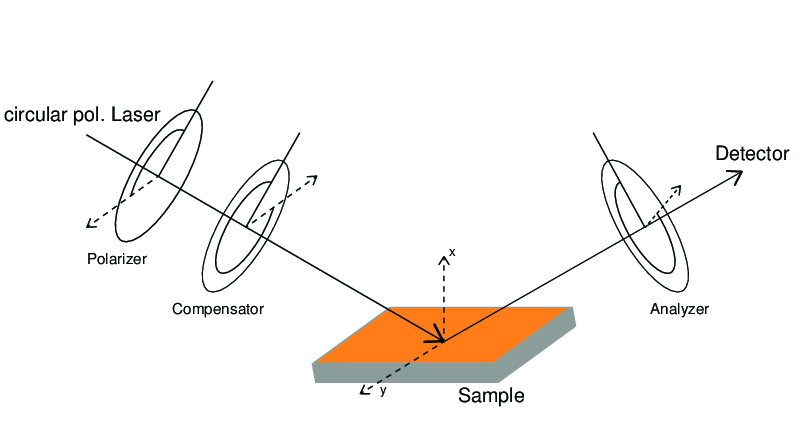
\includegraphics[width=6in]{Ellipsometer-in-a-PCSA-configuration.png}
\caption{PCSA ellipsometer in reflection mode \cite{Kurz}.}
\label{fig:PCSAellipsometer}
\end{center}
\end{figure}

\begin{figure}[htbp]
\begin{center}
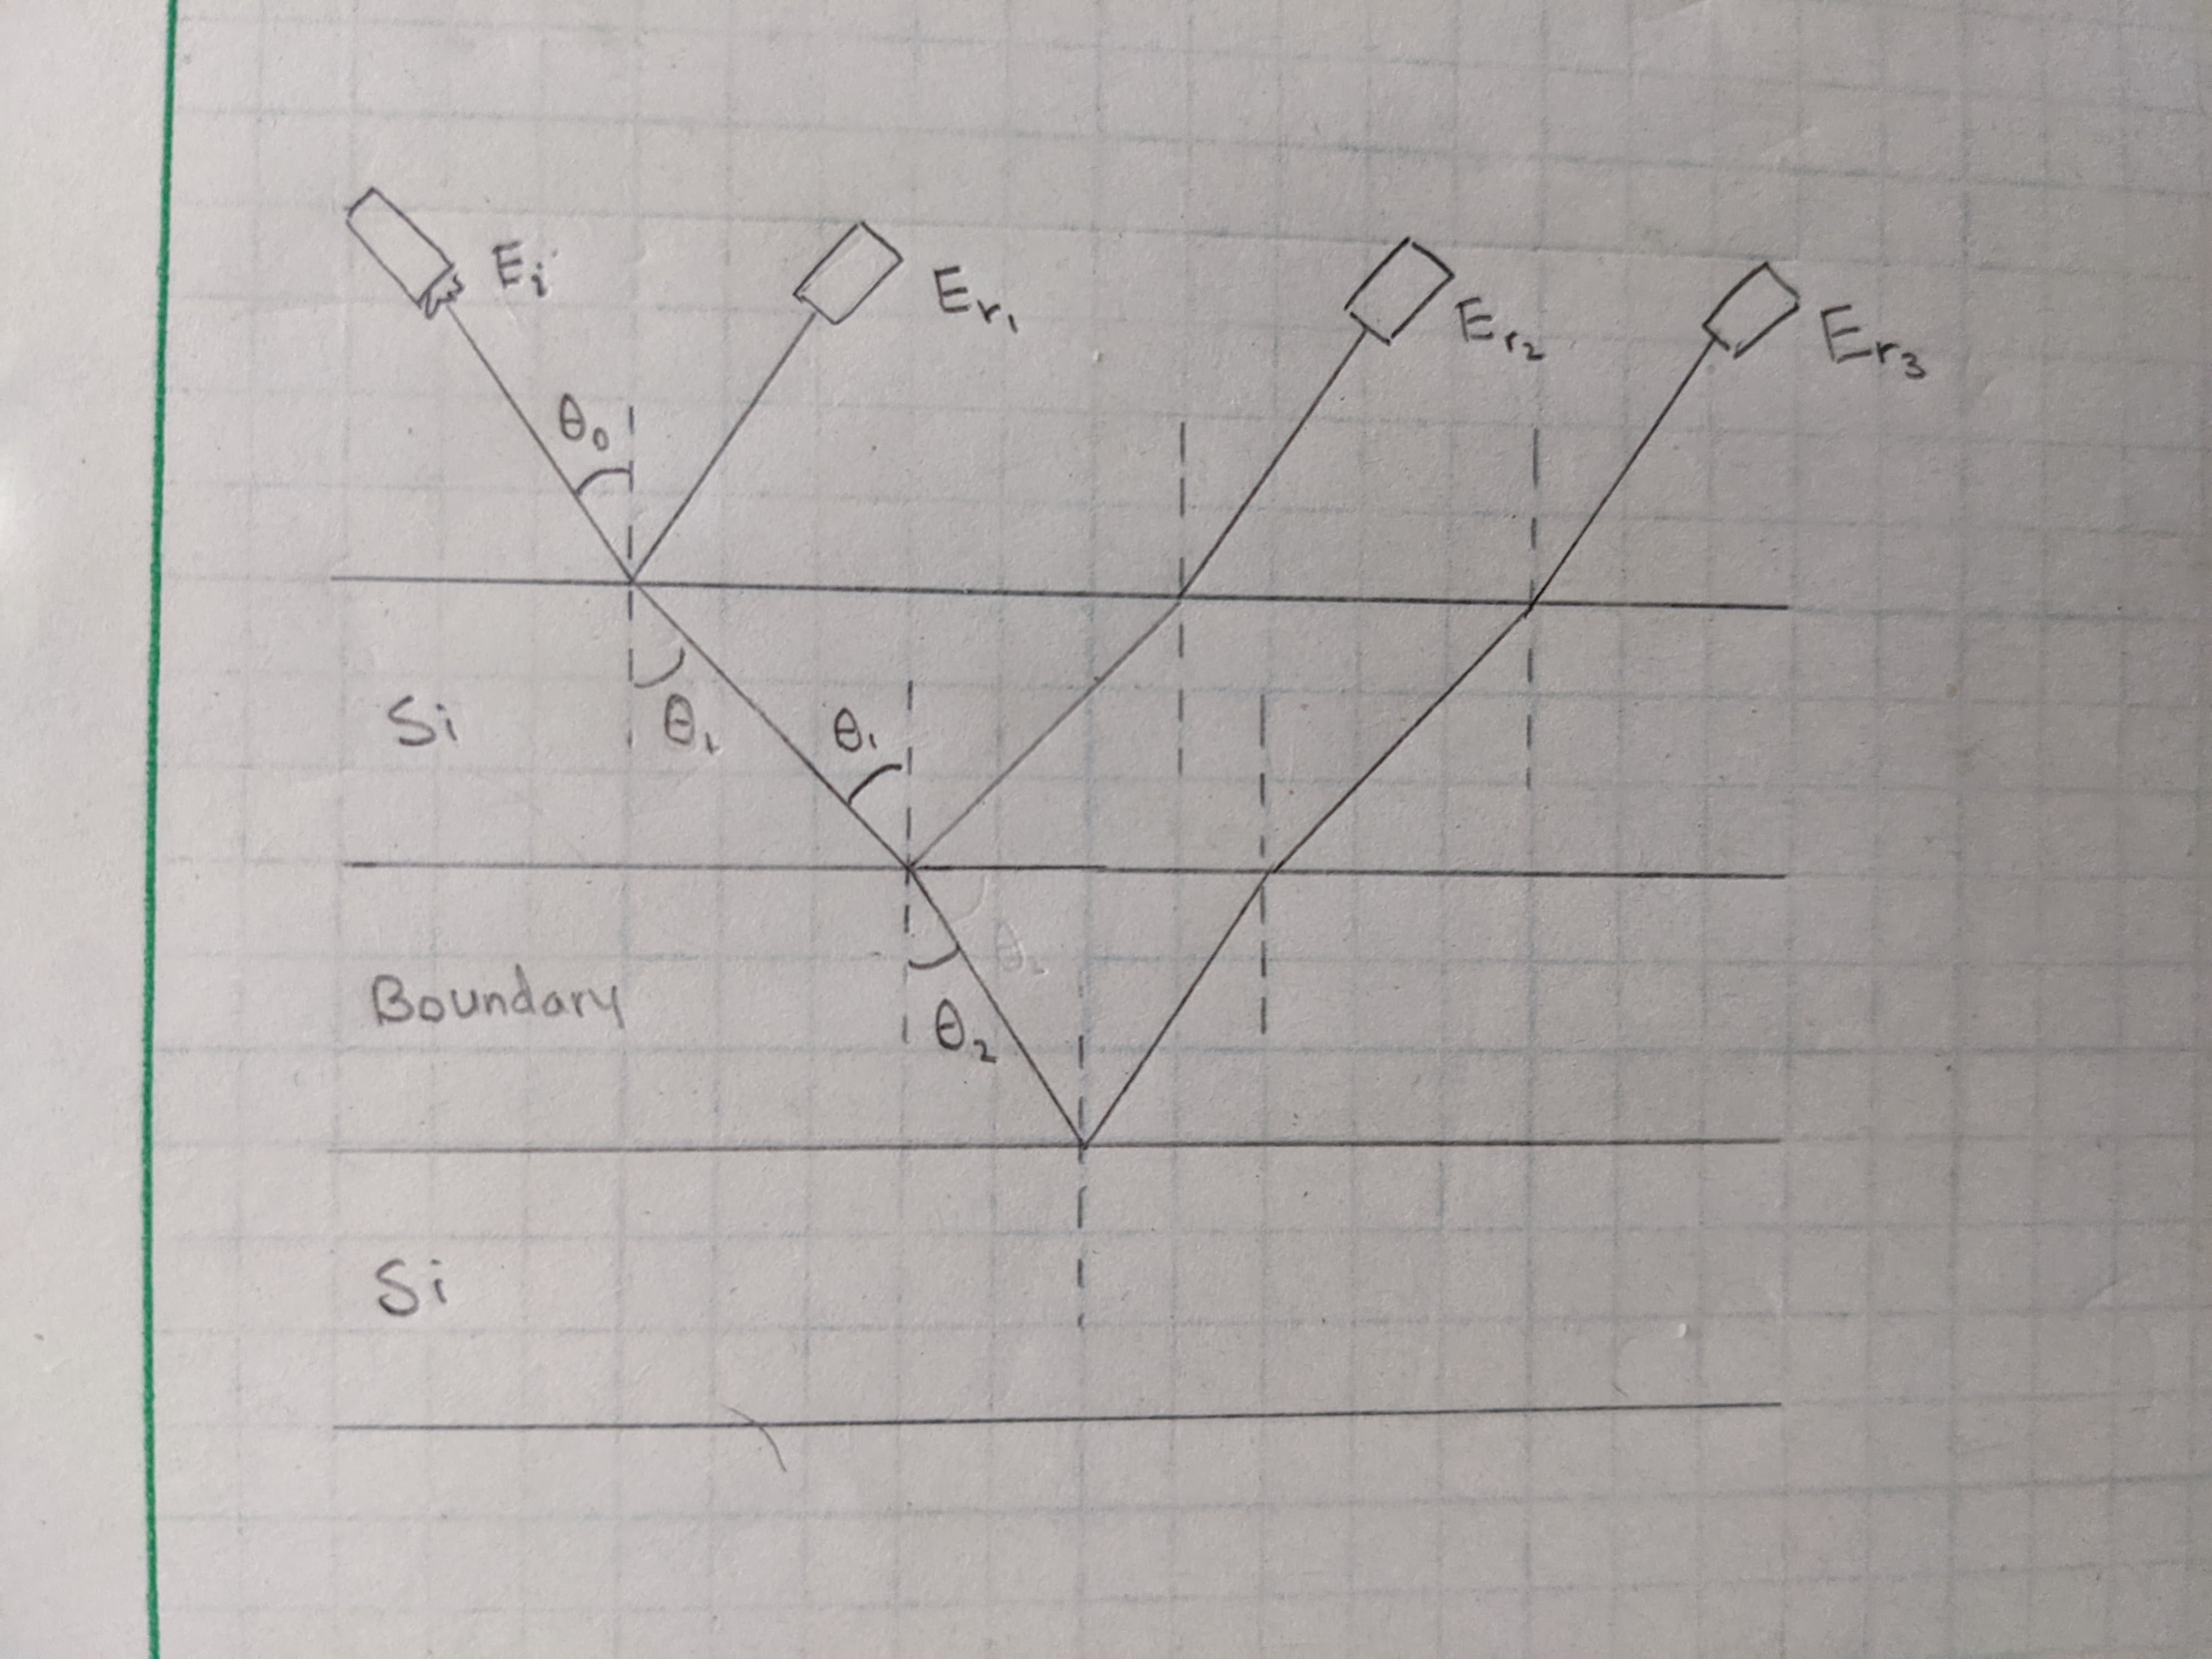
\includegraphics[width=6in]{my_ellipsometry.jpg}
\caption{Adapting figure \ref{fig:PCSAellipsometer} for multiple layers. Optical pieces like the polarizer and compensator are not shown.}
\label{fig:myellipsometer}
\end{center}
\end{figure}

\newpage

Basic parts list:

\begin{enumerate}
    \item Laser source
        \begin{itemize}
        \item It will be 1550 nm.
        \item I may be able to replace it with an IR LED.
        \end{itemize}
    \item Linear polarizer
    \item Compensator (optional?)
        \begin{itemize}
        \item "Introduces a defined phase retardation of one field component with respect to the orthogonal field component, the sample S, the analyzer A, and a detector" \cite{Kurz}.
        \item I am a bit confused on what this part does, to be frank. It appears to be optional for reasons that I do not understand.
        \end{itemize}
    \item Sample
        \begin{itemize}
        \item I believe I will be able to use the same size wafers as the shear strength experiment. As I will elucidate after this list, I have been struggling with doing the exact math, so this is just based on reading a several papers which used OOM 10mm x 10m x 1mm thin films.
        \end{itemize}
    \item Detector
\end{enumerate}

Actually putting this technique into practice is not straightforward---at least for someone like me who does not have an abundance of experience with experimental optics, although based on the papers I read, this does appear to be a difficult problem in general. The math is all linear algebra, but due to the number of variables, actually doing the calculations is quite overwhelming, especially when I am struggling to understand what is happening conceptually. Having an unknown index of refraction and an unknown thickness adds a lot of complexity to the problem, and some sources imply that it may not be able to resolve both values, or you may only be able to find a relative value \cite{Zawada}. There are also limits to capabilities of ellipsometry, as the changes in index of refraction may be so small that they are virtually undetectable \cite{Kalkowski}. The diagram in Figure \ref{fig:PCSAellipsometer} is also considered the simplest case; due to the complexity of my specific experiment, I may need to use a more complicated form of ellipsometry.

\subsection{Mechanical q}

In progress...

\begin{thebibliography}{9}
    
	\bibitem{Helie}
	  Hélie, David, et al.,
	  \emph{Reinforced direct bonding of optical materials by femtosecond laser welding}.
	  Applied optics 51.12 p.2098-2106 (2012).    

	\bibitem{Ohlidal}
	  He, Mengfei, and Sidney R. Nagel,
	  \emph{Ellipsometry of layered systems}.
	  Optical Characterization of Thin Solid Films. Springer, Cham, p.233-267 (2018).

	\bibitem{Kurz}
	  Kurz, Volker Luiz Siegmar.,
	  \emph{Orientation, conformation and phase transitions of thin polymer films and self-assembled monolayers studied by SFG spectroscopy}.
	  Diss. (2010).

    \bibitem{Zawada}
	  Zawada, A.,
	  \emph{Determining the refractive index, absolute thickness and local slope of a thin transparent film using multi-wavelength and multi-incident-angle interference}.
	  Optics Express 28.16 p.24198-24213 (2020).
  
    \bibitem{Kalkowski}
	  Kalkowski, Gerhard, et al.,
	  \emph{Glass-glass direct bonding}.
	  ECS Transactions 64.5 p.3 (2014).
 
\end{thebibliography} %Must end the environment

\end{document} 